\chapter{Dynamic Schedule}

\section{Aim}

The aim is to choose a schedule of customer arrivals times that minimises the expected cost of the system. The expected cost is a linear combination of the total customers' waiting time and the server's idle time. Instead of choosing a fixed schedule at the start of service as is common in literature, the schedule will be chosen progressively. Immediately after a customer arrives and begins waiting for service, the scheduler chooses the arrival time of the next customer.

\section{Assumptions}

To simplify this problem, need to make several assumptions:
\begin{itemize}[nosep]
	\item Service times are independent and identically distributed (iid)
	\item Each service time has an exponential distribution with mean service time $\mu$
	\item There is a single server
	\item The queue operates on a first in, first out (FIFO) basis
	\item Customers can be scheduled to arrive at any future (or present) time
	\item Customers are punctual and arrive at their scheduled time
\end{itemize}

\section{List of Variables}

\begin{tabularx}{\textwidth}{c c X}
	$\mu$ & : & mean service time of each customer \\
	$c_{W}$ & : & cost of customer's waiting time per unit time \\
	$c_{I}$ & : & cost of server's idle time per unit time \\
	$k$ & : & current number of customers waiting \\
	$j$ & : & number of customers waiting immediately after the next customer's arrival \\
	$n$ & : & number of customers remaining to be scheduled \\
	$a$ & : & time next customer is scheduled to arrive (relative to current time) \\
	$C_{n}^{*} (k)$ & : & the expected cost of having $k$ customers waiting and $n$ customers remaining to be scheduled \\
	$C_{n} (a, k)$ & : & the expected cost of having $k$ customers waiting, $n$ customers remaining to be scheduled and the next customer scheduled to arrive after $a$ time units \\
	$p_{a} (k, j)$ & : & the probability of transitioning from $k$ customers waiting to $j$ customers waiting after $a$ time units if the next customer is scheduled to arrive after $a$ time units \\
	$R_{a} (k, j)$ & : & the expected cost of transitioning from $k$ customers waiting to $j$ customers waiting after $a$ time units if the next customer is scheduled to arrive after $a$ time units
\end{tabularx}

\section{Objective Function}

The state $(n, k)$ refers to $n$ customers remaining to be scheduled and $k$ customers in the queue waiting for service. The time the next customer is scheduled to arrive is $a$, and the number of customers waiting for service immediately after that customer's arrival is $j$. The expected cost at the current state is a function of the expected cost involved in transitioning to the next state, the expected cost at the next state and the probability of transitioning to the next state over all possible next states. 

The expected cost of the state $(n, k)$ where $n \geq 1$ is given by the following form of Bellman's equation:
\begin{equation} \label{Bellman}
	C_{n}^{*} (k) = \min_{a \geq 0} C_{n} (a, k) = \min_{a \geq 0} \left[ \sum_{j = 1}^{k + 1} p_{a} (k, j) \Big( R_{a} (k, j) + C_{n - 1}^{*} (j) \Big) \right]
\end{equation}

Equation \ref{Bellman} is a recursive equation involving $C^{*}$. The optimal solution is found by solving for each customer's arrival time $a$ iteratively. The optimal policy $a^{*}$ is the customer's arrival time that attains the minimum cost whereby
\begin{equation} \label{Left-Closed}
	C_{n}^{*} (k) = C_{n} (a^{*}, k) = \min_{a \geq 0} C_{n} (a, k)
\end{equation}

It is reasonably intuitive that the minimum cost cannot occur at $a = \infty$. As $a \to \infty$, the probability that the server becomes idle converges to $1$. In addition, the expected idle time of the server converges to $\infty$. As the cost of the server's idle time $c_{I}$ is strictly positive, the overall expected cost must also converge to $\infty$ as $a \to \infty$. Thus, $\displaystyle \lim_{a \to \infty} C_{n} (a, k) = \infty$.

Consider the set of possible policies $\mathcal{A}$ given by
\begin{equation}
	\mathcal{A} = \{ 0 \} \bigcup \left\{ a > 0 : \frac{\partial}{\partial a} C_{n} (a, k) = 0 \right\}
\end{equation}

Solving Equation \ref{Left-Closed} involves solving a nonlinear optimisation problem over a left-closed interval. This solution is equivalent to the solution found by checking the left end point (where $a = 0$) and all points where $\frac{\partial}{\partial a} C_{n} (a, k) = 0$. Thus, the the optimal policy can be found by solving
\begin{equation}
	C_{n}^{*} (k) = \min_{a \in \mathcal{A}} C_{n} (a, k)
\end{equation}

As will be explained later, it is not possible to find a `nice' closed form for $\frac{\partial}{\partial a} C_{n} (a, k)$ for general $n$ and $k$. However, for given values of $n$ and $k$, it is reasonably efficient to solve $\frac{\partial}{\partial a} C_{n} (a, k) = 0$. Thus, the expected cost can be found by computing $\frac{\partial}{\partial a} C_{n} (a, k)$ for each state $(n, k)$. Of course, this method becomes more computationally inefficient, the larger the number of states.

\subsection{Base Case}

Finding the solution iteratively requires a solution for the base case where $n = 0$. If $n = 0$, there are no customers remaining to be scheduled, which implies the server will not be idle for the remaining of service. The cost of state $(0, k)$ (i.e., the base case) is thus the summation of the waiting cost of the $k$ customers in the queue.

Let $w_{i}$ be the expected waiting time of the customer that is currently in position $i$ in the queue, and $c_{W}$ be the cost of the customers' waiting time per unit time. The cost of the base case is thus given by
\begin{align*}
 	C_{0}^{*} (k) & = c_{W} \sum_{i = 2}^{k} w_{i} + c_{S} \sum_{i = 1}^{k} \mu \\
 	& = c_{W} \sum_{i = 2}^{k} \mu (i - 1) + c_{S} k \mu \\
 	& = \frac{c_{W} \mu k (k - 1)}{2} + c_{S} k \mu
\end{align*}

Scale $C_{0}^{*} (k)$ by dividing by $(c_{S} + c_{W})$ and substituting $\gamma = \frac{c_{S}}{c_{S} + c_{W}}$:
\begin{equation}
	C_{0}^{*} (k) = (1 - \gamma) \cdot \frac{\mu k (k - 1)}{2} + \gamma k \mu
\end{equation}

\subsection{Transition Probability}

Let $S_{i}$ be the service time of the customer that is currently in position $i$ in the queue. The service times $S_{1}, \ldots, S_{n}$ are iid (independent and identically distributed) exponential random variables with mean $\mu$.

For $r \geq 1$, the waiting time of the customer in position $(r + 1)$ in the queue is:
\begin{equation}
	X = \sum_{i = 1}^{r} S_{i} \sim \text{Erlang}(j, \mu)
\end{equation}

which has the pdf:
\begin{equation}
	f (x; r) = \frac{1}{\mu \cdot (r - 1)!} \left( \frac{x}{\mu} \right)^{r - 1} \exp \left( \frac{-x}{\mu} \right)
\end{equation}

Let $W_{t}$ be a Poisson Point Process with $W_{t} \sim \text{Poisson} \left( \frac{t}{\mu} \right)$. For $r \geq 1$, the probability that the customer currently in position $(r + 1)$ in the queue waits longer than $a$ time units before service is equal to the probability that $W_{a}$ is smaller than $r$, such that
\begin{equation}
	\mathbb{P} (X > a) = \mathbb{P} (W_{a} < r)
\end{equation}

The transition probability $p_{a} (k, j)$ is the probability that the queue length changes from $k$ customers initially to $j$ customers on the arrival of the next customer after $a$ time units. In other words, it is the probability that there are $k - (j - 1)$ departures from the queue over a time interval of length $a$. Computing this probability requires the cdf of the Erlang distribution, which is calculated (for $a > 0$) as follows:
\begin{align*}
	F (a; r) & = \mathbb{P} (X \leq a) \\
	& = 1 - \mathbb{P} (X > a) \\
	& = 1 - \mathbb{P} (W_{a} < r) \\
	& = 1 - \sum_{i = 0}^{r - 1} \mathbb{P} (W_{a} = i) \\
	& = 1 - \sum_{i = 0}^{r - 1} \frac{1}{i!} \left( \frac{a}{\mu} \right)^{i} \exp \left( \frac{-a}{\mu} \right)
\end{align*}

Moreover, $F (0; r) = \mathbb{P} (X = 0) = 0$ by definition. Therefore, the cdf of the Erlang distribution is defined as
\begin{equation}
	F (a; r) = \begin{cases} 1 - \sum_{i = 0}^{r - 1} \frac{1}{i!} \left( \frac{a}{\mu} \right)^{i} \exp \left( \frac{-a}{\mu} \right) & \text{where $a > 0$} \\ 0 & \text{where $a = 0$} \end{cases}
\end{equation}

Can now compute the transition probability on a case by case basis. The full derivation is included in the appendix and only the final equation is presented here.
\begin{equation}
	p_{a} (k, j) = \begin{cases}
		\mathbbm{1} (j = 1) & \text{where $k = 0$} \\
		F (a; k) & \text{where $k \geq 1, j = 1$} \\
		F (a; k - j + 1) - F (a; k - j + 2) & \text{where $k \geq 1, 2 \leq j \leq k$} \\
		1 - F (a; 1) & \text{where $k \geq 1, j = (k + 1)$} \\
		0 & \text{otherwise}
	\end{cases}
\end{equation}

\subsection{Expected Transition Cost}

The cost involved in transitioning from state $(n, k)$ to state $(n - 1, j)$ in $a$ time units is a linear combination of the expected total waiting time of the customers during the transition and the expected total server availability time during the transition as in Chapter 3. During the transition, the server is available for the entire time interval, so the total server availability time during the transition is always $a$.

The expected total waiting time of the customers depends on the conditional expectation of the Erlang distribution, which is derived here (for $a > 0$).
\begin{align*}
	G (a; k) & = \mathbb{E} [X | X \leq a] \\
	& = \int x \cdot \mathbb{P} (X \in dx | X \leq a) \\
	& = \int x \cdot \frac{\mathbb{P} (X \in dx, X \leq a)}{\mathbb{P} (X \leq a)} \\
	& = \frac{1}{F (a; r)} \int_{0}^{a} x \cdot f(x; r) dx \\
	& = \frac{1}{F (a; r)} \int_{0}^{a} x \cdot \frac{1}{\mu \cdot (r - 1)!} \left( \frac{x}{\mu} \right)^{r - 1} \exp \left( \frac{-x}{\mu} \right) \\
	& = \frac{\mu r}{F (a; r)} \int_{0}^{a} \frac{1}{\mu \cdot r!} \left( \frac{x}{\mu} \right)^{r} \exp \left( \frac{-x}{\mu} \right) \\
	& = \mu r \cdot \frac{F (a; r + 1)}{F (a; r)}
\end{align*}

In addition, $G (0; r) = \mathbb{E} [X | X \leq 0] = 0$ by definition. Therefore, the conditional expectation of the Erlang distribution is defined as
\begin{equation}
	G (a; r) = \begin{cases} \mu r \cdot \frac{F (a; r + 1)}{F (a; r)} & \text{where $a > 0$} \\ 0 & \text{where $a = 0$} \end{cases}
\end{equation}

This expression for the conditional expectation makes intutive sense. The mean of the Erlang distribution is $\mathbb{E} [X] = \mu r$. In addition, $\forall a > 0$, $\frac{F (a; r + 1)}{F (a; r)} < 1$. Thus, $\forall a > 0$, $\mathbb{E} [X | X \leq a] < \mathbb{E} [X]$ as expected. Moreover, 
\begin{equation}
	\lim_{a \to \infty} \frac{F (a; r + 1)}{F (a; r)} = \frac{\displaystyle \lim_{a \to \infty} F (a; r + 1)}{\displaystyle \lim_{a \to \infty} F (a; r)} = \frac{1}{1} = 1
\end{equation}

Thus, $\displaystyle \lim_{a \to \infty} \mathbb{E} [X | X \leq a] = \mathbb{E} [X]$ as expected.

In a similar way to the transition probability, the expected transition cost is derived on a case by case basis. The per unit time cost of the customers' waiting time and the server's idle time are $c_{W}$ and $c_{I}$ respectively. The full derivation is included in the appendix and the final equation is presented here.
\begin{multline}
	R_{a} (k, j) \\
	= \begin{cases}
		\gamma a & \text{where $k \in \{ 0, 1 \}$} \\
		(1 - \gamma) \cdot \frac{G (a; k) (k - 1)}{2} + \gamma a & \text{where $k \geq 2, j = 1$} \\
		(1 - \gamma) \left[ a (j - 2) + \frac{G (a; k - (j - 1)) [k - (j - 2)]}{2} \right] + \gamma a & \text{where $k \geq 2, 2 \leq j \leq k$} \\
		(1 - \gamma) \cdot a (j - 2) + \gamma a & \text{where $k \geq 2, j = (k + 1)$}
	\end{cases}
\end{multline}

\section{Example Models}
\subsection{State (3, 2)}

Assume that the mean service time $\mu$ is $1$. In addition, assume that the per unit time costs of the customers' waiting time and server's idle time ($c_{W}$ and $c_{I}$ respectively) are both $1$. Under these assumptions, the cost of state $(3, 2)$ for various values of $a$ is given by the following expression, which is continuous for $a \geq 0$.

\begin{equation*}
	C_{3} (a, 2) =
	\begin{cases}
 		9.88121 & \text{where $a = 0$} \\
 		\frac{\mathrm{e}^{-a} \left( \mathrm{e}^{a} a (2.29362 - 0.5 a) - (0.5 a + 3.29362) a - 1.15888 \mathrm{e}^{a} + (a + 5.52005) \mathrm{e}^{2 a} - 4.36117 \right)}{\mathrm{e}^{a} - 1} & \text{where $a > 0$}
	\end{cases}
\end{equation*}

This equation is plotted for $a \in [0, 10]$ to visualise the relationship between the cost and $a$. The resulting figure is Figure \ref{Graph_3_2}.

\begin{figure}[htb]
	\centering
	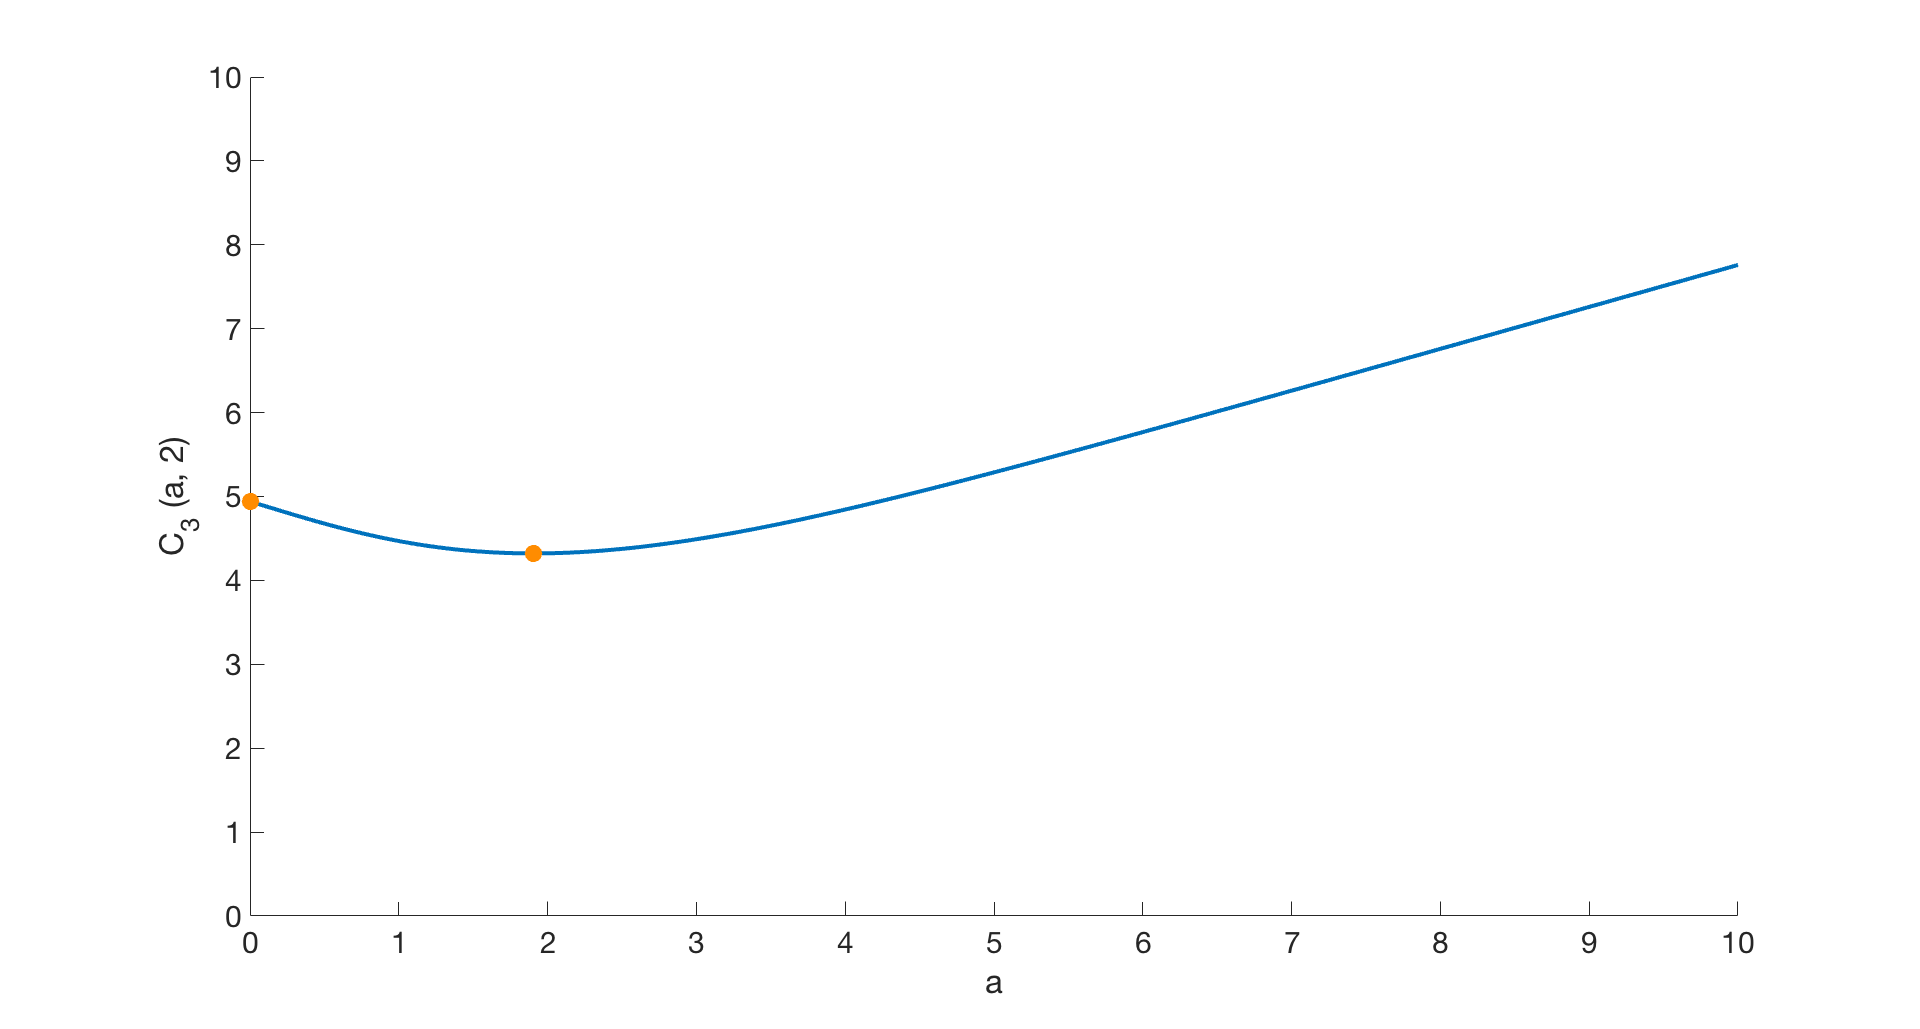
\includegraphics[width = 0.85\textwidth]{Graph_3_2.png}
	\caption{Cost of state with n = 3, k = 2 for various values of a}
	\label{Graph_3_2}
\end{figure}

The only value of $a$ where $\frac{\partial}{\partial a} C_{3} (a, 2) = 0$ is $1.90481$. Thus, the set of possible policies $\mathcal{A}$ is $\{ 0, 1.90481 \}$ whereby there are two possible policies labelled as orange dots on Figure \ref{Graph_3_2}. Moreover, note that as $a$ increases beyond 2, the cost increases approximately linearly as the expected waiting time of the next customer and the expected idle time of the server both increase linearly.

The optimal policy $a^{*}$ that minimises $C_{3} (a, 2)$ is $1.90481$ where the cost is $8.64338$. If on arrival of a customer, there are $2$ customers in the queue and $3$ customers remaining to be scheduled, then the next customer should be scheduled to arrive in $1.90481$ time units. This is slightly below the expected service time of the two customers in the queue to account for the idle cost of the server.

\subsection{Model for Six Customers}

Assume there are 6 customers that need to be scheduled for service who all have a mean service time $\mu$ of 1. The initial state is $(6, 0)$, and the possible states during service are all states in the set

\begin{equation}
	\Big\{ (n, k) \in \{ 0, 1, \ldots, 6 \}^{2} : n + k \leq 6 \Big\}
\end{equation}

\begin{table}[htb]
	\centering
	\begin{tabular}{c c c || c | c | c | c | c | c | c}
		& & & \multicolumn{7}{c}{queue length ($k$)} \\
		& & & 0 & 1 & 2 & 3 & 4 & 5 & 6 \\ \hline \hline
		\parbox[t]{2mm}{\multirow{7}{*}{\rotatebox[origin=c]{90}{customers to be}}} & \parbox[t]{2mm}{\multirow{7}{*}{\rotatebox[origin=c]{90}{scheduled ($n$)}}} & 0 & 0 & 1 & 3 & 6 & 10 & 15 & 21 \\
		& & 1 & 1 & 2.69315 & 4.97937 & 8.04949 & 11.9605 & 16.7418 \\
		& & 2 & 2.69315 & 4.52005 & 6.81367 & 9.88121 & 13.7875 & \\
		& & 3 & 4.52005 & 6.35018 & 8.64338 & 11.7105 & & \\
		& & 4 & 6.35018 & 8.18013 & 10.4733 & & & \\
		& & 5 & 8.18013 & 10.0101 & & & & \\
		& & 6 & 10.0101 & & & & & \\
	\end{tabular}
	\caption{Cost of possible states for 6 total customers}
	\label{Cost_6_Customers}
\end{table}

Table \ref{Cost_6_Customers} displays the calculated expected costs for each possible state if there are 6 total customers (assuming $c_{W} = c_{I} = 1$). The cost of the initial state is $10.0101$, thus the expected cost of servicing six customers with an alterable schedule is $10.0101$.

Note that in this table, for $n \geq 1$, $C_{n}^{*} (0) = C_{n - 1}^{*} (1)$. This is due to the fact that if there are no customers currently waiting (e.g., initially), then it is always optimal to schedule the next arrival immediately. The expected cost thus doesn't change as the next arrival occurs immediately.

The worst state on this table is the state $(0, 6)$, which is all six customers waiting for serviced. This can occur if all six customers are scheduled to arrive immediately (to ensure no idle time), or the first customer has an extremely long service time.

\begin{table}[htb]
	\centering
	\begin{tabular}{c c c || c | c | c | c | c | c}
		& & & \multicolumn{6}{c}{queue length ($k$)} \\
		& & & 0 & 1 & 2 & 3 & 4 & 5 \\ \hline \hline
		\parbox[t]{2mm}{\multirow{6}{*}{\rotatebox[origin=c]{90}{customers to be}}} & \parbox[t]{2mm}{\multirow{6}{*}{\rotatebox[origin=c]{90}{scheduled ($n$)}}} & 1 & 0 & 0.693147 & 1.75711 & 2.82577 & 3.85505 & 4.8492 \\
		& & 2 & 0 & 0.826902 & 1.90223 & 2.95223 & 3.95872 & \\
		& & 3 & 0 & 0.83013 & 1.90481 & 2.95403 & & \\
		& & 4 & 0 & 0.82995 & 1.90455 & & & \\
		& & 5 & 0 & 0.829925 & & & & \\
		& & 6 & 0 & & & & & \\
	\end{tabular}
	\caption{Optimal policy for each possible states for 6 total customers}
	\label{Policy_6_Customers}
\end{table}

Table \ref{Policy_6_Customers} displays the corresponding arrival times for the costs in Table \ref{Cost_6_Customers}. This table does not include any optimal times for $n = 0$, as there is no next customer to schedule in those states.

The first pattern to notice is (as discussed earlier) if there are no customers currently waiting (i.e., $k = 0$), then the optimal solution is to schedule the next arrival immediately. This makes intutive sense as scheduling the next arrival immediately minimises the future idle time and ensures that the waiting time of the next customer is simpler their service time.

As $k$ increases for constant $n$, the optimal schedule time increases approxiimately proportionately. The optimal $a^{*}$ increases by approximately $\mu$ for each extra $k$ to minimise the waiting time of the next customer.

Finally, for $n \geq 1$, the value of $a^{*}$ such that $C_{n}^{*} (k) = C_{n} (a^{*}, k)$ is always less than $\mu k$ (i.e., the expected time for the queue to be empty). This is due to the cost of the idle time of the customer leading to the desire for the next customer to arrive just before the queue becomes empty.


































